\documentclass{article}

\usepackage{fancyhdr}

\usepackage{textcomp}
\usepackage{enumitem}
\usepackage{amsthm, amssymb,amsmath}
\usepackage{graphicx}
\usepackage{tabto}
\usepackage{url}
\usepackage{float}

\title{MATH 425 Fall 2024 Final Project: \\ Calculation of a Fundamental Matrix}
\date{Due: Sunday December 22, 2024}
\author{Miguel Antonio Logarta}

\pagestyle{fancy}

\fancyhead[L]{Math 425 Final Project}  % Left side of the header
\fancyhead[C]{Fall 2024}  % Center of the header
\fancyhead[R]{Due: Sunday December 22, 2024}  % Right side of the header (current date)


\newcommand\aug{\fboxsep=-\fboxrule\!\!\!\fbox{\strut}\!\!\!}

\begin{document}


\maketitle  % This command generates the title page.
\thispagestyle{fancy}

\section{Introduction}
In computer vision, using two cameras is a common way to understand the layout of a 3D scene. This approach solves the problem of missing information when using just one image. With a single image, a computer cannot accurately determine the 3D layout because it lacks details like depth and distance between objects. This is where epipolar geometry becomes important. \\

Epipolar geometry explains the relationship between two images taken from different positions by two cameras viewing the same 3D scene. The fundamental matrix is helpful in this context because it lets us reconstruct a 3D scene using two uncalibrated cameras. This can be done with just a few matching points between the two images, without needing additional information about the 3D scene.\\

Before we dive into the code, I'll first explain the basics of Epipolar Geometry.

\section{Epipolar Geometry}
\begin{figure}[H]
    \centering
    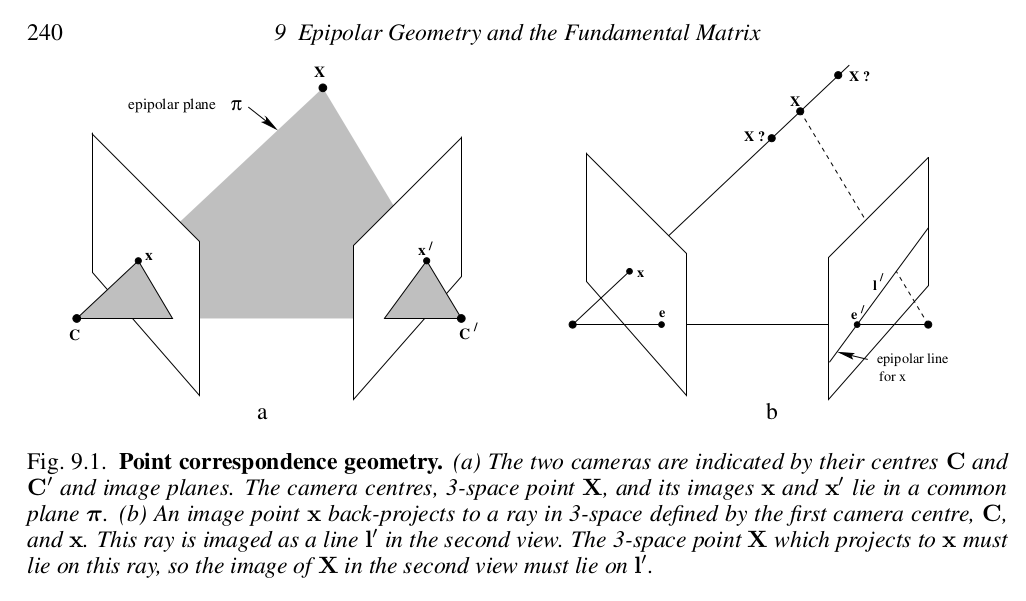
\includegraphics[width=1\textwidth]{epipolar_geometry.png}
\end{figure}

Imagine a 3D point in space called \textbf{X}, which is projected onto two images as points x and x'. Both x and x' lie on the same plane, called the epipolar plane. These images represent the views from two different cameras. \\

The points along the line connecting the 3D point \textbf{X} to x, as seen from camera \textbf{C}, create a line l' in the view of the other camera \textbf{C'}. This line l' is called an epipolar line. Similarly, the points connecting \textbf{X} to x', as seen from camera \textbf{C'}, form another epipolar line l in the view of camera \textbf{C}. \\

A key property of epipolar lines is that they intersect at specific points called epipoles, e and e'. These epipoles are the points where the line connecting the two camera centers (known as the baseline) intersects the image planes.

\section{The Fundamental Matrix}
The Fundamental matrix relates the corresponding points x and x' of the two cameras in which the epipolar lines are written as 
$$l' = [e']_{\times} H_{\pi} x = F x$$
$$l = [[e']_{\times} H_{\pi} x]^Tx' = F^Tx'$$
In short, it maps the points in one image to their corresponding epipolar lines in the other image. In addition, the explanation from the textbook also shows that the second camera is just a transformation of the first camera in the 3D scene. It satisfies the equation
$$x'^TFx = 0$$
where F is a 3x3 matrix.

\section{Calculating the Fundamental Matrix}

To find the fundamental matrix, we use the normalized eight point algorithm. The normalized eight point algorithm calculates the fundamental matrix with 8 matching point correspondences from two matching images. The algorithm from the textbook is as follows:
\begin{figure}[H]
    \centering
    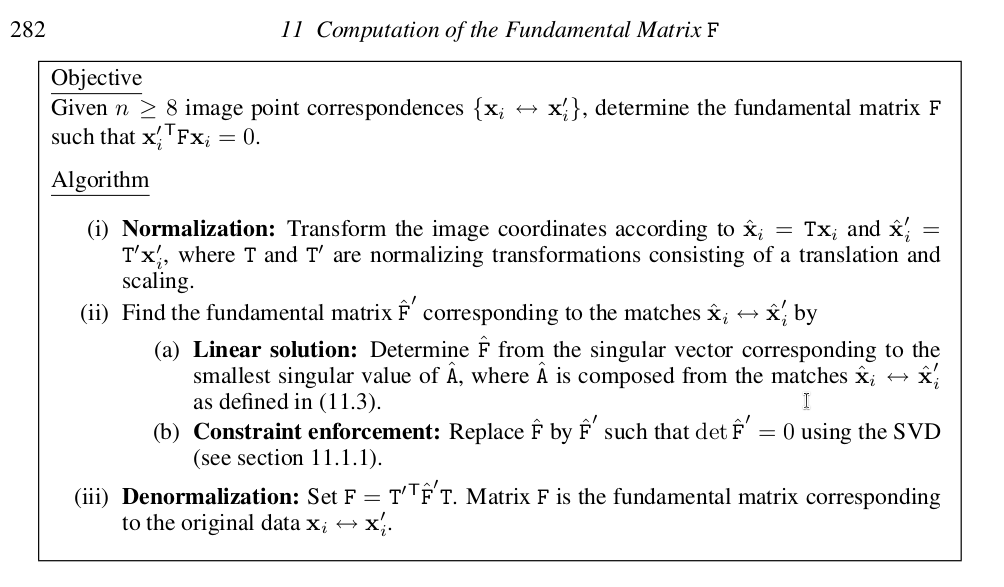
\includegraphics[width=1\textwidth]{eight_point_algorithm.png}
\end{figure}

\section{Translating Math Into Code}
\subsection{Getting Point Correspondences}
For this project, I used two images of my toaster to calculate the fundamental matrix. I manually selected 8 points from both images and stored the point correspondences in \textbf{x} and \textbf{x'} where each coordinate $x_i = (x,y,1)^T$ and $x_i' = (x',y',1)^T$. The points are highlighted in red.
\begin{figure}[H]
    \centering
    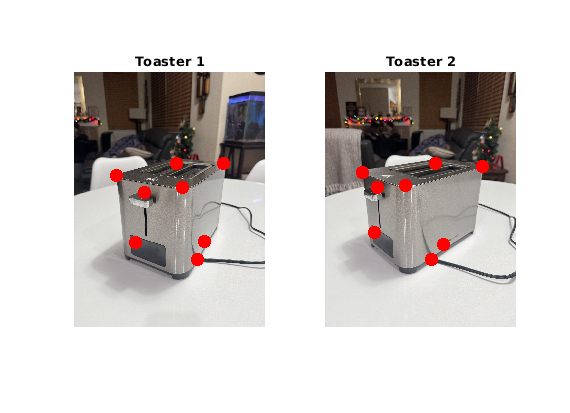
\includegraphics[width=1\textwidth]{point_correspondences.png}
\end{figure}

\subsection{Normalizing the Points}
Next, I needed to normalize the points. Normalization is an important step because modern cameras produce images with very large pixel values. Without normalization, these large numbers can make the calculation of the fundamental matrix less accurate. \\

The textbook recommended scaling each point using the RMS (root mean square) distance formula, where the origin of the points are centered around (0,0), with the average distance from the origin being $\sqrt{2}$. However, the explanation in the book lacked clear examples, so I had to research further. After some digging, I learned that each point should be scaled using the following formula:
$$
s = \left( \frac{2N}{\sum_{i=1}^N \|x_i - \bar{x}\|^2} \right)^{1/2}
$$

After some more digging, I used the scale to construct a transformation matrix T and applied it to every point in \textbf{x} and \textbf{x'}

$$
T = \begin{pmatrix}
    s & 0 & -s * \bar{x}\\
    0 & s & -s * \bar{y}\\
    0 & 0 & 1 
\end{pmatrix}
$$

\subsection{Main Algorithm}
These matching points are in \textbf{x} and \textbf{x'} where each coordinate $x_i = (x,y,1)^T$ and $x_i' = (x',y',1)^T$. We then try to solve for the system of linear equations $A\textbf{f} = \textbf{0}$:
$$
A\mathbf{f} =
\begin{bmatrix}
x'_1 x_1 & x'_1 y_1 & x'_1 & y'_1 x_1 & y'_1 y_1 & y'_1 & x_1 & y_1 & 1 \\
\vdots & \vdots & \vdots & \vdots & \vdots & \vdots & \vdots & \vdots & \vdots \\
x'_n x_n & x'_n y_n & x'_n & y'_n x_n & y'_n y_n & y'_n & x_n & y_n & 1
\end{bmatrix}
\mathbf{f} = 0.
$$ 

The linear solution \textbf{f} is found in the \underline{last column of $V^T$} in the SVD of A where $SVD(A) = UDV^T$. We end up with a 9x1 vector which we then have to reshape into a 3x3 matrix which is our Fundamental Matrix.\\

Now we have to enforce a constraint on F. F must be of rank-2 and singular ($det(F) = 0$). This ensures that the epipolar lines in both images meet at a common epipole.\\

To enforce this constraint, we get the SVD of F again where $SVD(F) = UDV^T$. We take the last diagonal of the 3x3 matrix D, and set it to zero to force F to be of rank 2. We recompute F' as F' = $F' = U * diag(r, s, 0) * V^T$ \\

\subsection{Denormalization}
We denormalize F by applying the transformation matrix T
$$F = T' * F' * T; $$

\section{Results}
Now that we have the fundamental matrix, we can plot the epipolar lines on both of our images. Since we denormalized F, we apply F to our denormalized coordinates instead of our normalized coordinates. The equations for our epipolar lines are:
$$l' = F x$$
$$l= F^Tx'$$

\begin{figure}[H]
    \centering
    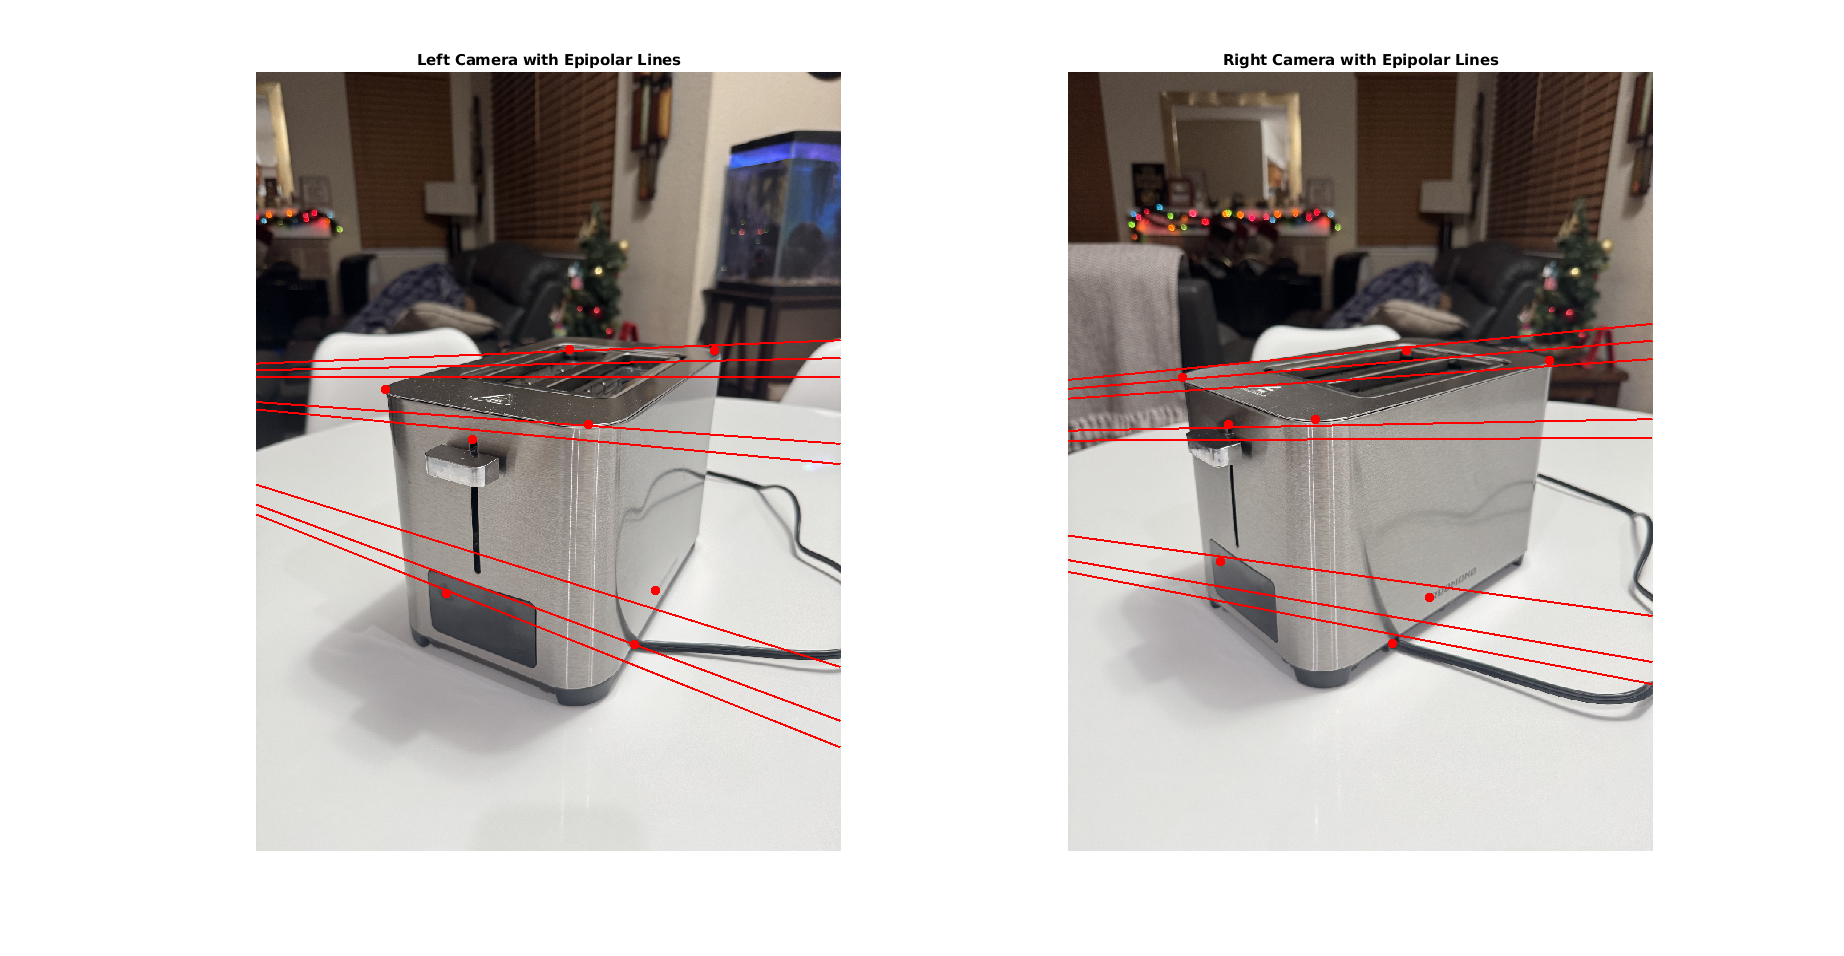
\includegraphics[width=1\textwidth]{results.png}
\end{figure}

\section{Remarks}
Here are the results. Unfortunately, while some of my epipolar lines align with the corresponding points, many of them do not. I believe this is due to an inaccurate fundamental matrix. When checking x'Fx=0x'Fx=0, the value was around 0.002, which might not be precise enough. After reviewing my code to ensure the correspondence points were properly normalized and the transformation was applied correctly, I couldn't find the issue before the deadline.\\

For future work, I plan to learn how the RANSAC algorithm works so it can automatically select key points in both images. I would also like to include examples where the cameras are parallel (so the epipolar lines are parallel) and a case where the epipole is inside the image, as the previous example showed the epipole outside the image.


\begin{thebibliography}{2}
    \bibitem{texbook}
    Hartley, Richard, and Andrew Zisserman. Multiple View Geometry in Computer Vision. Cambridge University Press, 2004. \\
    Chapter 9, 10, and 11 are the main sources of information regarding the calculation of the Fundamental matrix. It contains a very detailed background of epipolar geometry complete with proofs and algorithms. 

    \bibitem{website}
    Hata, Kenji, and Silvio Savarese. “CS231A Course Notes 3: Epipolar Geometry.” Stanford.Edu, \url{web.stanford.edu/class/cs231a/course_notes/03-epipolar-geometry.pdf}. Accessed 23 Dec. 2024. \\ 
    This is an external source that contains information on epipolar geometry. I used this source due to its simplified explanation of epipolar geometry and the eight-point algorithm.

\end{thebibliography}
\end{document}
